%preamble
\documentclass[letterpaper]{article}
\synctex=1
\usepackage{graphicx}
\graphicspath{ {images/} }

\usepackage{lipsum}
\usepackage{float}
% \bibliographystyle{IEEEtran}
\bibliographystyle{ieeetr}

\usepackage{amssymb}

\usepackage{siunitx}
%actual document
\begin{document}

  % \maketitle %insert titlepage here
  \begin{titlepage}
    \begin{center}
        \vspace*{1cm}
        \Huge
        Experiment 2
        \vspace{1cm}

        Measurements of e/m for Electrons
        \vspace{1cm}

        By: Arun Woosaree
        \vspace{1cm}

        Lab partners:
        \vspace{.25cm}
        \Large

        % Fatemeh Ghafari Far
        Purvish Jajal

        % Yvonne Hong
        % \vspace{1cm}

        \Huge
        PHYS 230 Lab EH71
        \vspace{1cm}

        TA: Andrei Tretiakov
        \vspace{1cm}

        Date of Lab: \today
        \vfill
    \end{center}
\end{titlepage}

\section{Introduction}
% Begin with experiment’s objectives\\
% Give physical background:\\
% ○ Describe investigated/used\\
% phenomena e.g. Gauss’s law,\\
% field lines, equipotential lines.\\
% ○ Do not copy text from a
% textbook/manual\\
% Provide equations you used\\
% ○ Identify all symbols\\

In this experiment, we measure the charge to mass ratio $e/m$ of electrons fired in a
Helmholtz coil.
The electrons are emmitted from a hot filament, accelerated by an electric field, and then deflected
by a magnetic field into a circular orbit. If the radius of this orbit is known,
as well as the intensity of the magnetic field, and the accelerating potential of the
electric field, we can determine $e/m$ and the velocity $v$ of the electrons, and an approximate value for
the earth's magnetic field $B_E$. Using the left-hand-rule for moving charge (since we are
dealing with electrons), we can also figure out the direction of the magnetic field which deflects the electrons.
The charge to mass ratio is found using the following equation, of which a derivation exists in the Discussion section.
The equation below is also linearized, and graphed, from which we obtain an approximate value of the earth's magnetic field
\begin{equation}
  \frac{e}{m} = \frac{2V}{(B_H-B_E)^2r^2}
\end{equation}
In this equation, $e$ is the charge of an electron, and $m$ is the mass of the electron, XXXXXXXXXXXXXXXXXX`V' is the AC voltage
, $B_H$ is the magnetic field of the coil, given by
\begin{equation}
  B_H=\frac{8\mu_0 NI}{ \sqrt{125} R}
\end{equation}
and r is the orbit radius of the electrons. In Equation 2 above, $\mu_0$ is the permeability permeability of free space,
$N$ is the number of turns in the Helmholtz coil, $R$ is the radius of the coil, and $I$ is the measured current through the
coil.

% we map electric potential and the electric field of a parallel plate capacitor.
% A capacitor is essentially two charged conductors separated by some insulator.
% In Part 1, we measure the potential differences in the region between the charged conductors in a circular capacitor,
% and since our geometry is simple, the electric potential can be compared with
% predictions made using Gauss's Law. In Part 2, we make a contour map consisting of equipotential
% curves from our data, which can then be used to construct the corresponding electric field lines
% of the parallel plate capacitor.
% By analyzing field patterns, we can determine the charge distribution on the surface of
% the charged conductors.

% In this ecperiment,
%
% The electric field \textbf{E} is defined such that a positive test charge $q$
% placed in the electric field will experience a force $\textbf{F}=q\textbf{E}$.
% Additionally, a certain amount of work $W=F \Delta s=qE\Delta s$ is done to move the charge
% a distance $\Delta s$, parallel to the electrostatic force. The electrostatic force is
% conservative, so the potential energy $U$ must decrease by $\Delta U=-qE\Delta s$.
% $V$, the electric potential is defined to be potential energy per unit charge $V=U/q$.
% The magnitude of an electric field at a point can be related to $V$ by
% \begin{equation}
%   E=-\frac{\Delta V}{\Delta s} \label{eq1}
% \end{equation}
%
% Using Gauss's law, in part 1 of the experiment we imagine a Gaussian cylinder enclosing
% the inner and outer conductors of a circular capacitor. This cylinder has a radius $r$ and
% length $L$ with flat end caps. Since \textbf{E} is parallel to the end caps, the flux, denoted $\Phi$ on
% the end caps are zero, which leaves the curved surface of the cylinder, with area $2\pi rL$.
% Since \textbf{E} is constant and perpendicular to the curved surface, the total flux $\Phi_E$ can be found
% \begin{equation}
%   \Phi_E = \Phi_{end1} + \Phi_{cylinder} + \Phi_{end2} = 0+E(2\pi rL) + 0 =\frac{Q}{\epsilon_0}
% \end{equation}
%
% $\sigma$ is defined as the charge per unit area on the surface of the inner conductor.
% The enclosed charge $Q$ enclosed by the Gaussian cylinder is $Q=(2 \pi AL)\sigma$, where
% $A$ is the radius of the inner conductor, and $\epsilon_0=8.85418782 \times 10^{-12} m^{-3} kg^{-1} s^{4} A^{2}$ is the permittivity of free space.
% Given the above information, the magnitude of the electric field at some radius $r$
% can then be computed
%
% \begin{equation}
%   E=\frac{\sigma A}{\epsilon_0 r}
% \end{equation}
%
% If we put a probe at radius $r$, and the outer conductor has a radius $B$ then the voltage
% difference between the probe and the outer conductor is
% \begin{equation}
%   V_r-V_B=\frac{\sigma A}{\epsilon_0 r} \ln{\frac{B}{r}}
% \end{equation}
% From which we can obtain the following equation if we set the voltage difference between the two conductors to have a value $V_0$
% \begin{equation}
%   \frac{V_r-V_B}{V_0}=\frac{\ln{\frac{B}{r}}}{\ln{\frac{B}{A}}}
% \end{equation}
% or alternatively,
% \begin{equation}
%   \ln{r} =\ln{\frac{A}{B}}(\frac{V_r-V_B}{V_0}) + ln{B}
% \end{equation}
% In part 2 of the experiment, we map the electric field of a parallel plate capacitor, and draw equipotential lines
% which correspond to electric field lines. An equipotential surface is defined such that the
% potential difference is constant at any point on the surface.


\section{Experimental Method}
% List all equipment used\\
% ○ Provide parameters as detailed as
% possible: masses, frequencies,
% etc.\\
% Report what YOU DID to achieve
% experimental goals:\\
% ○ Do not use imperative clause\\
% ○ Use first person narrative or
% passive voice\\
% Based on this section you should be
% able to reproduce your results without a
% manual

\textbf{List of Equipment:}
\begin{itemize}
  \item Helmholtz coil apparatus (Figures 1 and 2)
  \item AC Voltage Source
  \item DC Voltage Source
  \item Voltmeter
  \item Ammeter
  \item Wires
\end{itemize}

\begin{figure}[h!]
    \centering
    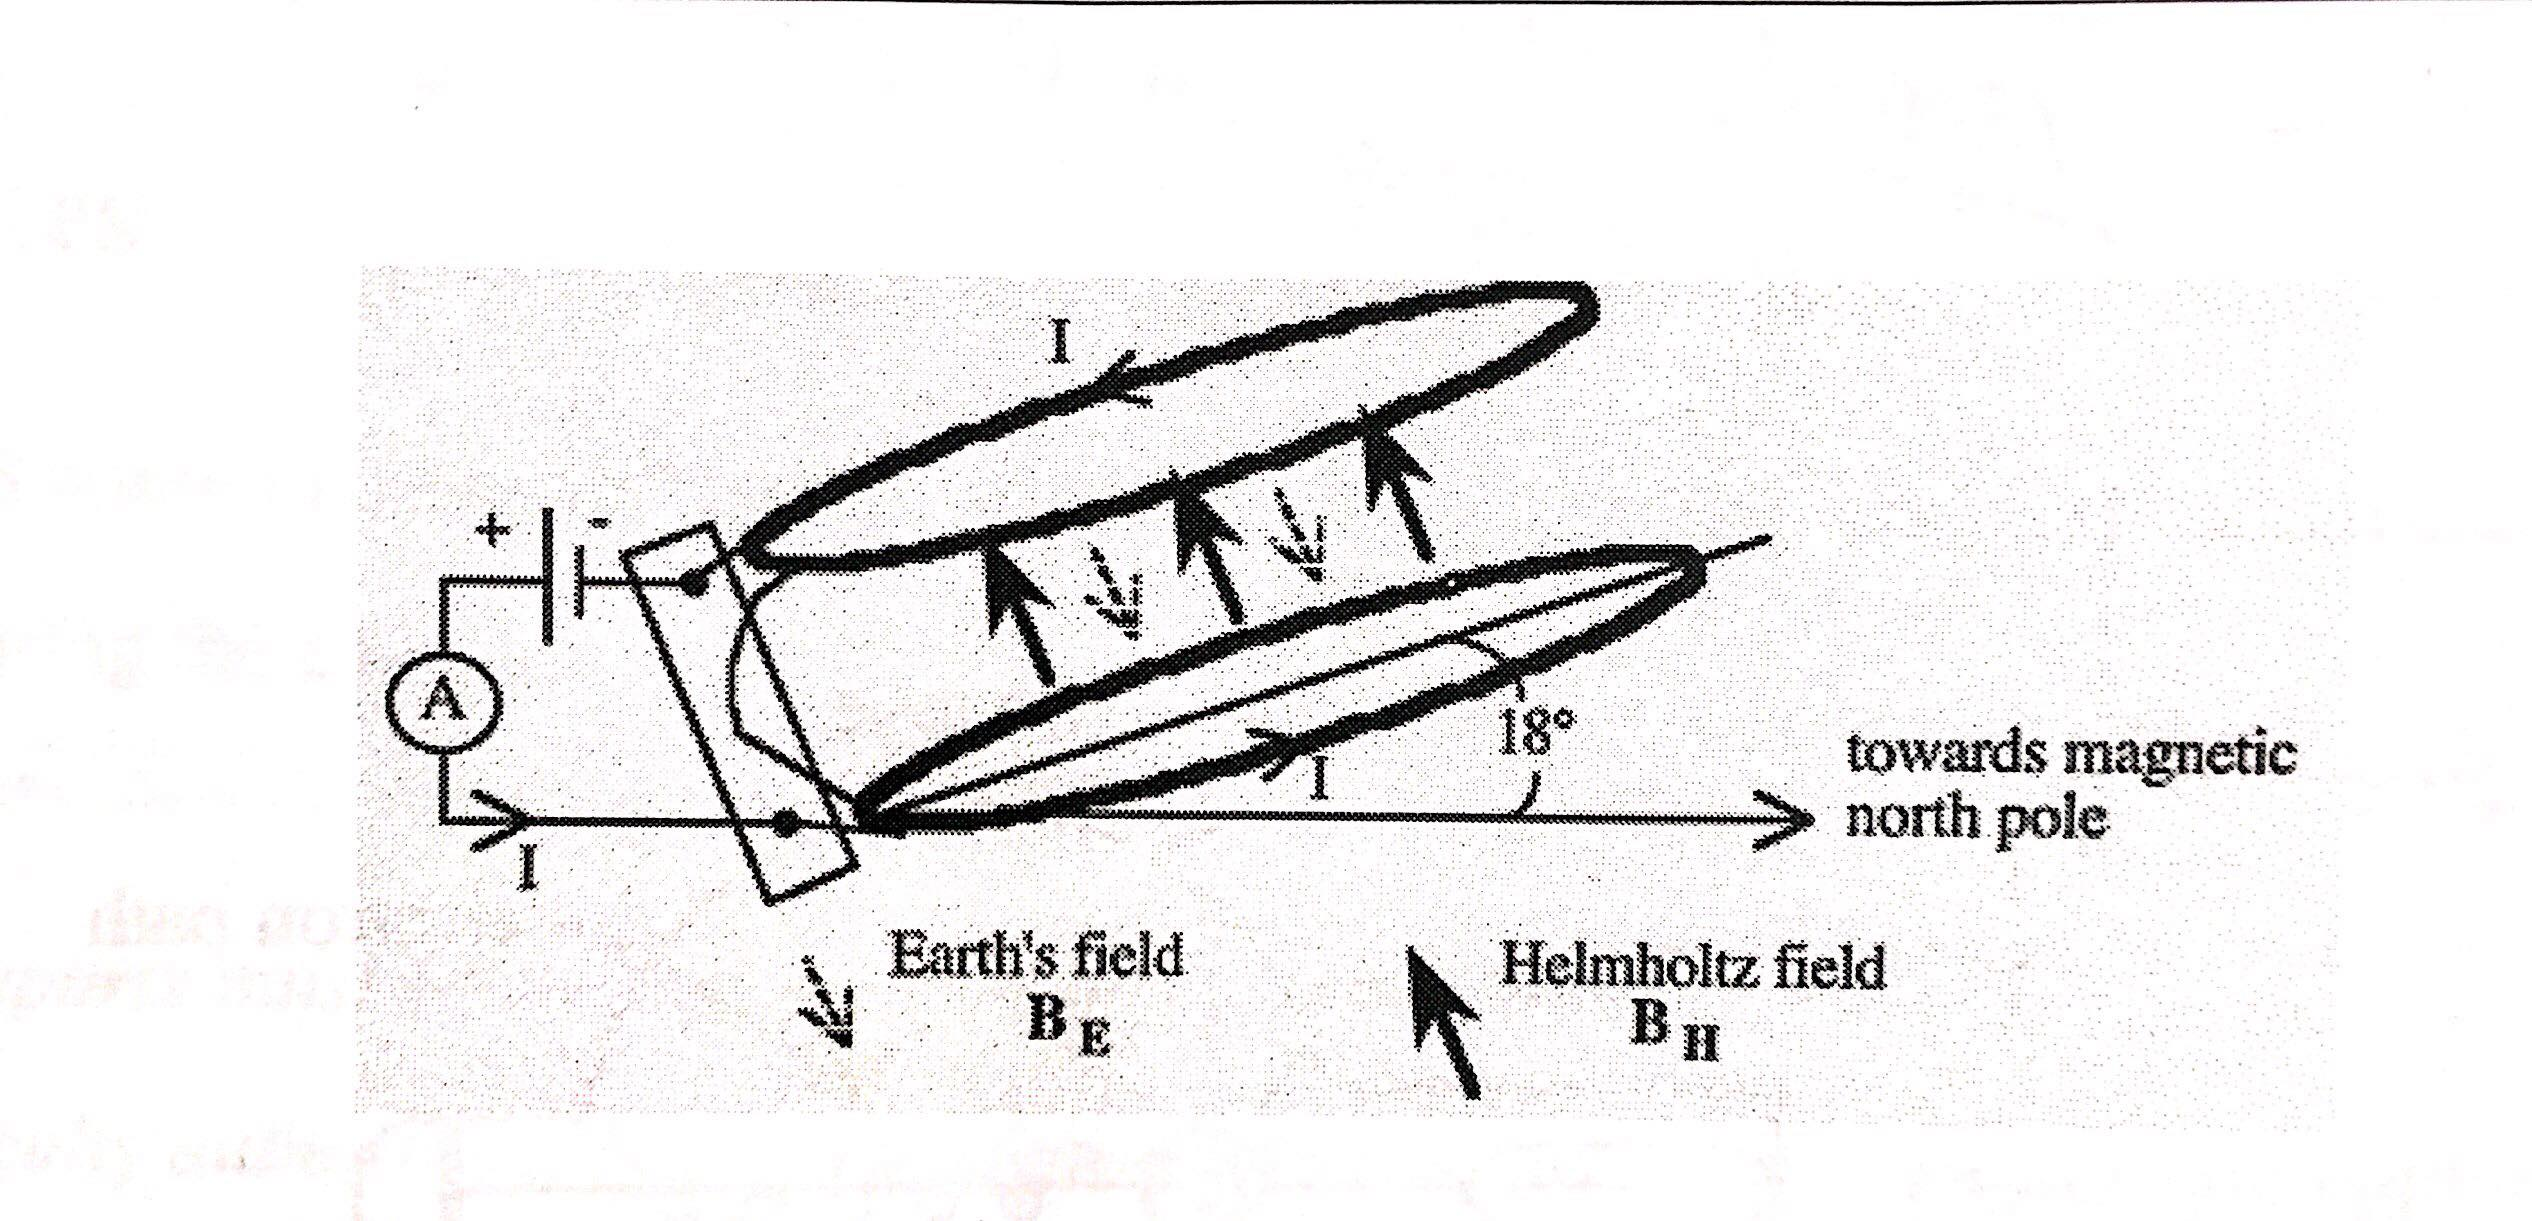
\includegraphics[width=\textwidth]{fig1.jpg}
    \caption{Helmholtz coil apparatus, and its alignment opposite to earth's magnetic field. \cite{labmanual}}
\end{figure}

The Helmholtz coil was set up such that its alignment is approximately
opposite to the Earth's magnetic field, which in Edmonton means that the coil
should be tilted upwards at an angle of about 18 degrees relative to the horizontal.

The apparatus involves three separate electrical circuits.
The filament, anode circuit, and the Helmholtz circuit are connected as outlined
below in Figure 2.
\begin{figure}[h!]
    \centering
    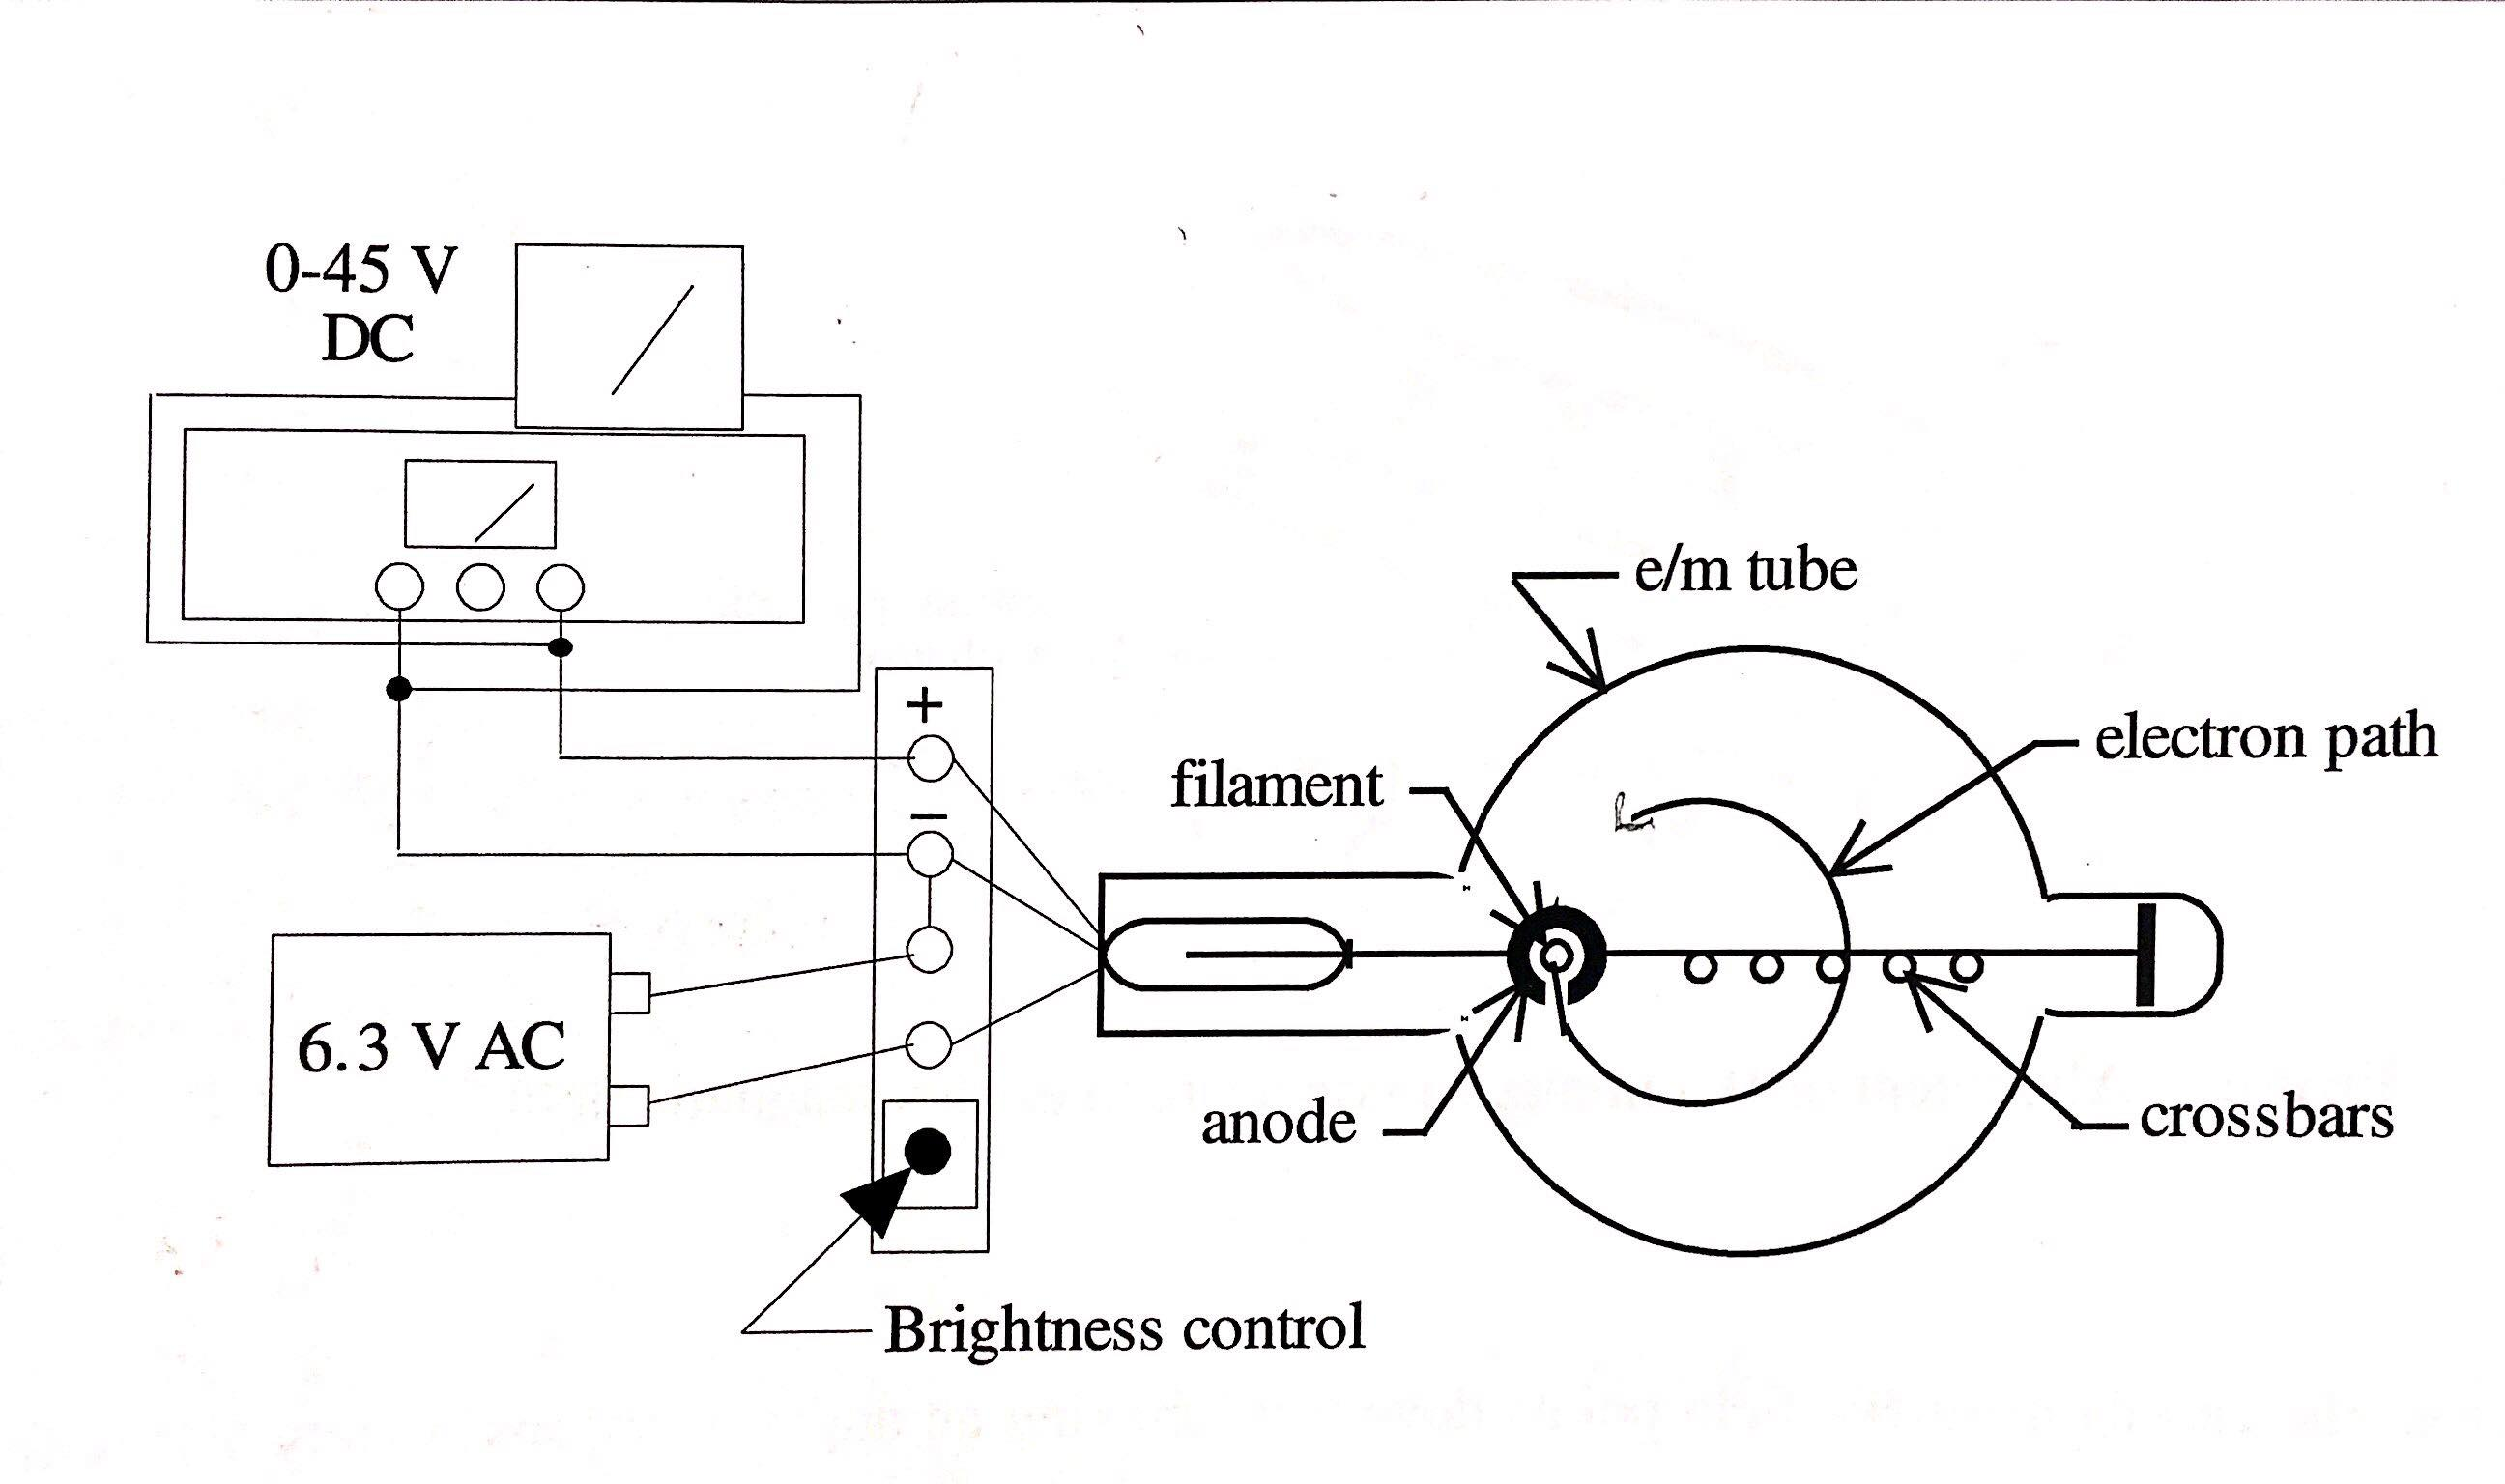
\includegraphics[width=.9\textwidth]{fig2.jpg}
    \caption{Circuit wiring for the apparatus \cite{labmanual}}
\end{figure}


% \subsection{Part 2}
% In Part 2 of the experiment, a circuit was constructed using the parallel plate capacitor.
% The positive end of the power supply was connected to one plate of the capacitor, and the negative
% lead of the power suppply was connected to the side of the capacitor with markings for measuring potential
% differences, and the negative end of the voltmeter. The probe remained connected to the positive end of the
% voltmeter, as in Part 1. Once again, the probe was touched at various points on the capacitor, and the
% voltage differences were recorded in a spreadsheet, from which Figures 5 and 6 were produced.
%
% % \begin{figure}[H]
%   \centering
%   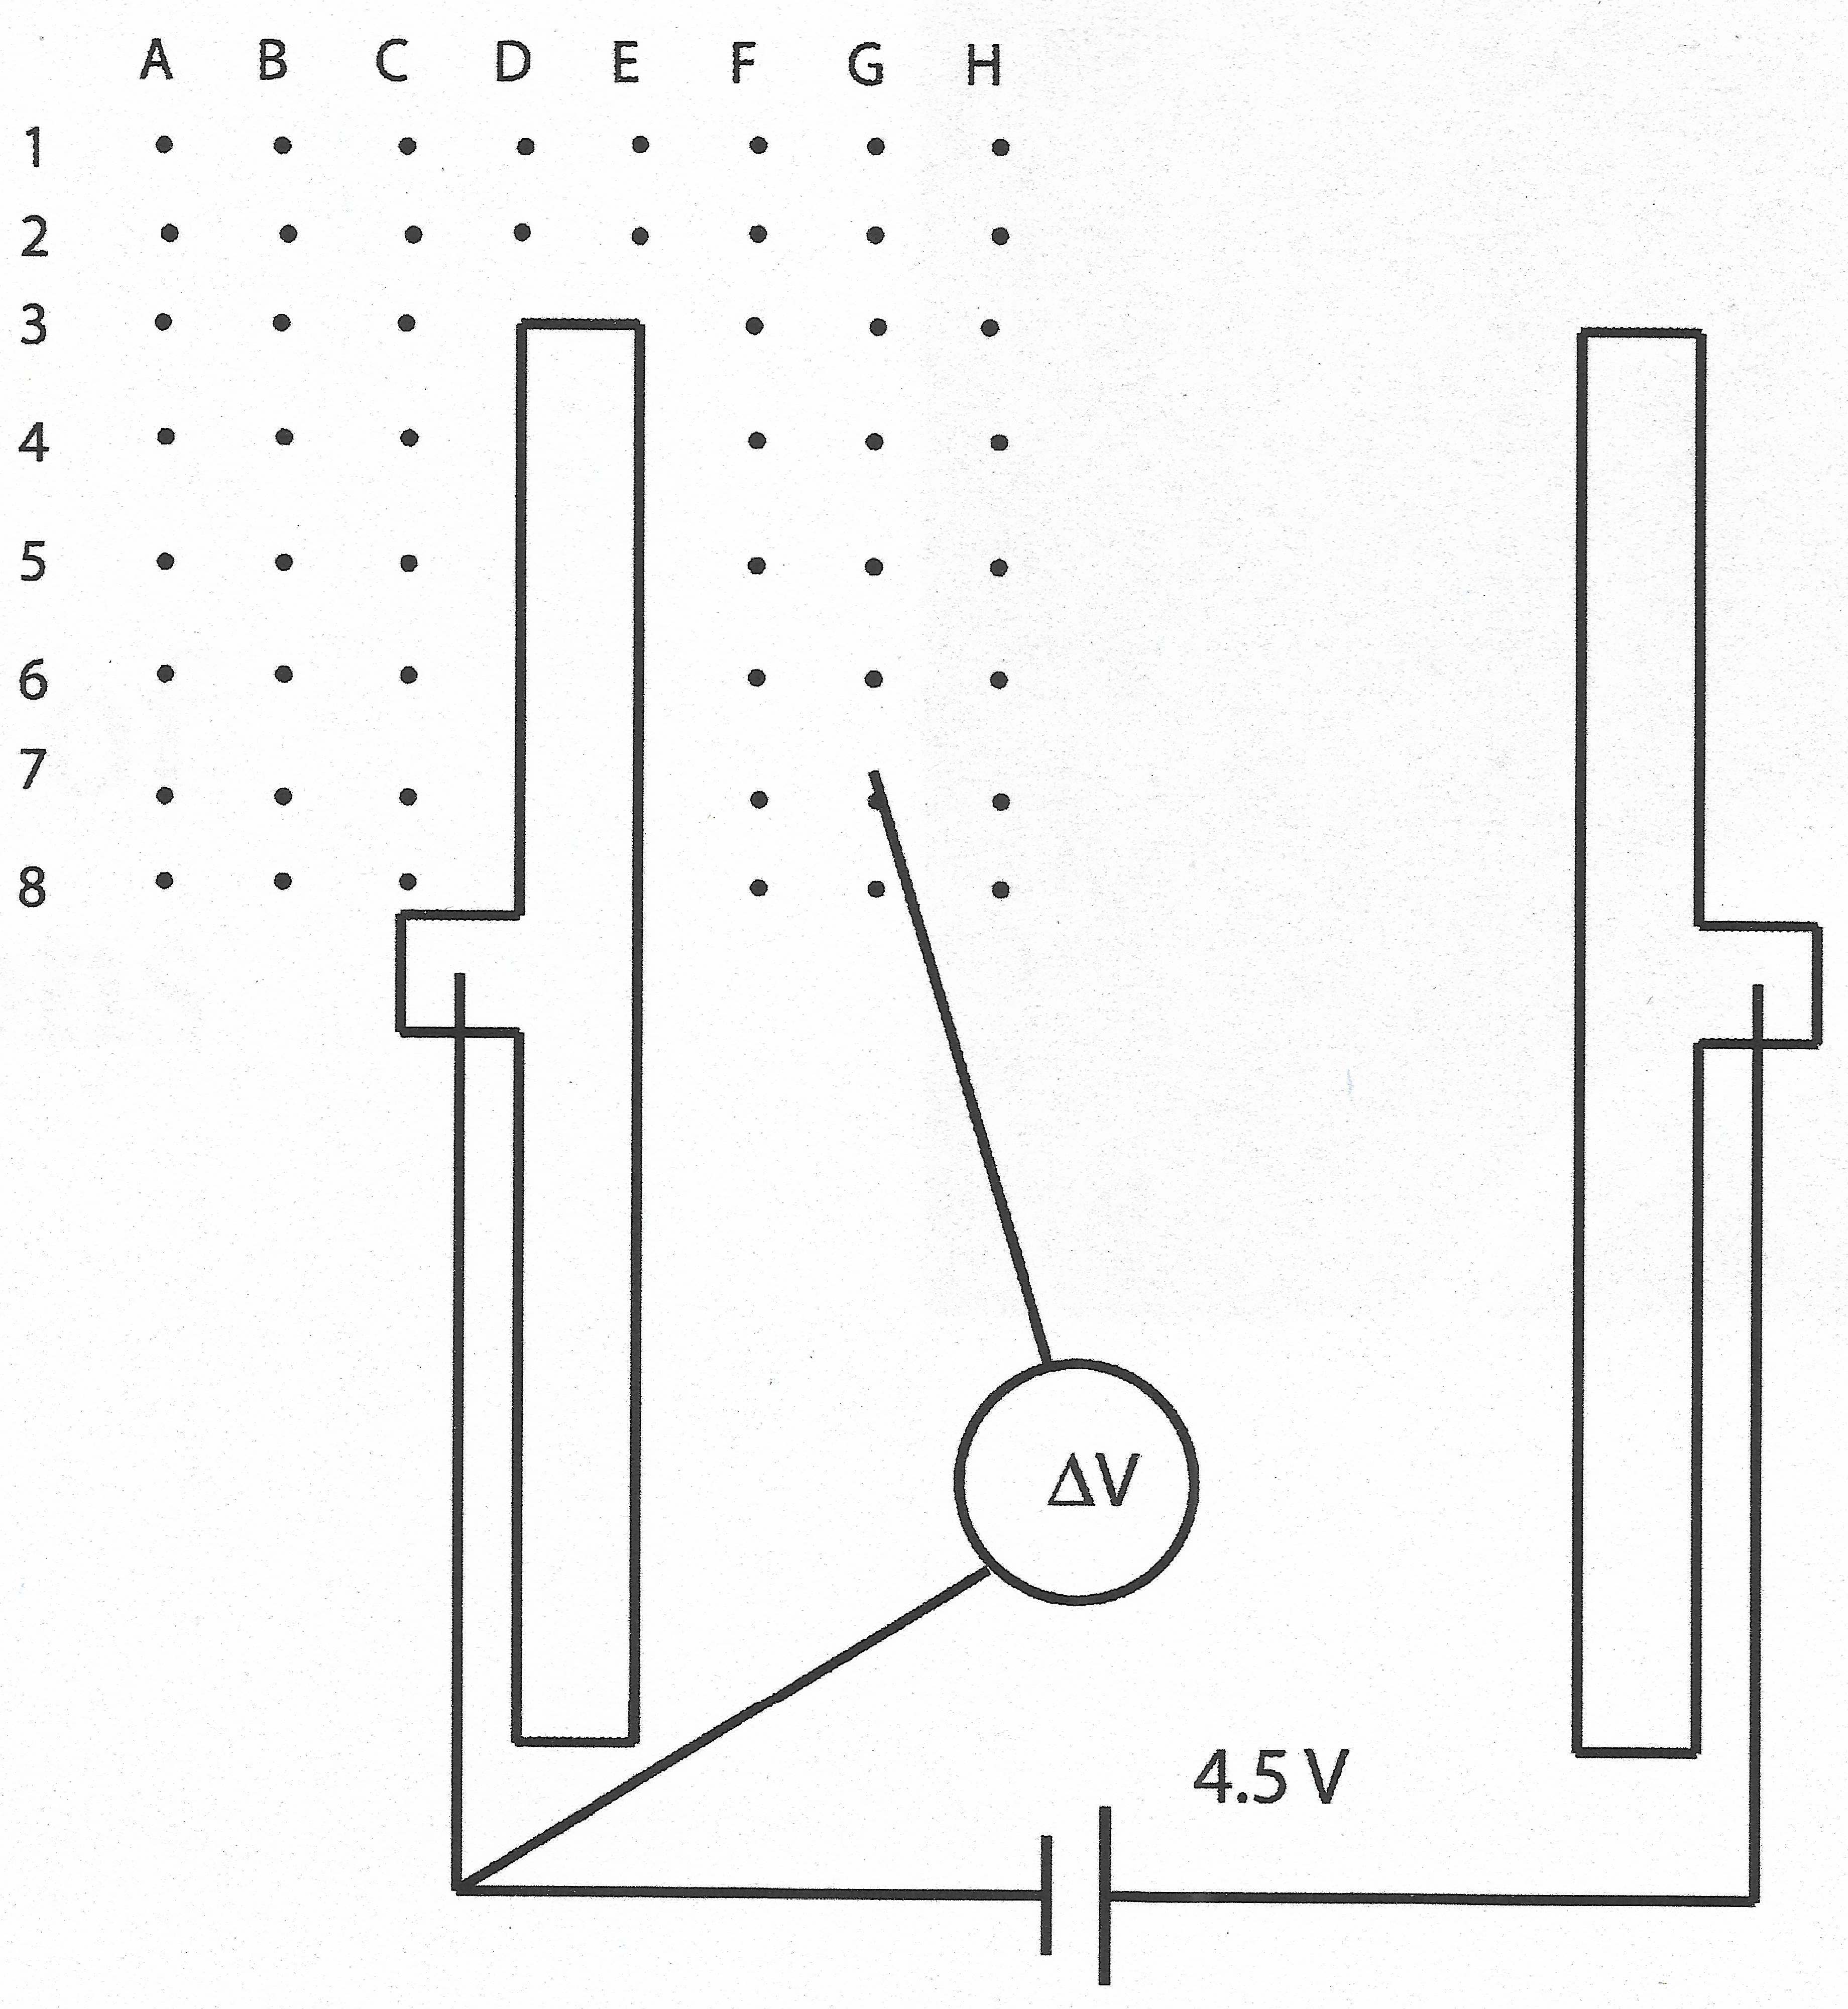
\includegraphics[width=.7\textwidth]{fig3.jpg}
%   \caption{Measuring the voltage difference in a region between two parallel conductors. \cite{labmanual}}
% \end{figure}

% When the apparatus illustrated above is set up, i.e. the lengths ‘r’ and ‘R’ are known, the center of the spark tape is marked when the bob is hanging freely at rest, and the bob is at the starting position, being held by the electromagnet, and the string is steadied to lessen any vibrations, the power going to the electromagnet is cut, and as a result, the bob is released from rest. The ‘RUN’ button on the spark timer is immediately (as best as humanly possible) held down, until the bob reaches approximately the maximum height on the other side of the track, or when one half of the period of the pendulum is completed.
%
% The spark timer is set to spark 30 times a second, so the time elapsed between each burn hole on the spark tape is 1/30th of a second. Once the spark tape is obtained from the apparatus, we need to measure the displacements of the glider as it was moving. To do so, we use a meter stick, and a displacement of 0.00m is taken to be the at the center of the spark tape, which is the point that was marked while the bob hangs freely at rest. This means that the initial displacement of the bob is taken to be a negative displacement, and the points after the bob passes the center are taken to be positive.
%
% After measuring the displacements of the bob, we enter the data points into Excel, and also calculate the time elapsed for each data point. (Ex. At the 10th burn hole, the time elapsed would be 10*1/30 seconds). From this data, we can calculate EK , EP , and ET  using equations  5,9 and 10 and plot them on a graph as a function of time. The ET curve was fit to a linear regression, and the EK and EP curves were fit to quadratic curves.

\section{Results}


% Should be a coherent text\\
% Present all data and calculations with words. Examples:\\
% ○ “Row data for free-fall acceleration measurements is given by Table 1.”\\
% ○ “In order to find the acceleration we plot doulbed distance as a function of
% time squired as is shown by Figure 1.” or “To find the acceleration we
% linearize Equation 1 as d(x)=ax, where x=t2/2 and plot it on Figure 1”.\\
% ○ “The slope of the graph corresponds to the acceleration and can be found
% along with the uncertainty using LINEST(see Table 2)”\\
% ○ “The uncertainty in distance is calculated as d= x+ y”\\
% ○ “Finally, the acceleration due to gravity is 9.81± 0.03 m/s2 ”\\
% All figures and should have label and caption \\(e.g. “Figure 1: position as a function
% of time during free fall”).\\
% Use scientific notation (103, not 1E3) and appropriate significant digits

\subsection{Part 1}
% Part I\\
% Linearized equation: provide
% all parameters e.g. variables,
% slope, intercept, etc.\\
% Linear graph: add trendline,
% provide fitting parameters
% (slope, intercept)\\
% Give values A and B obtained
% from the graph and measured
% directly\\
% Use Linest to find
% uncertainties\\

Raw data recorded while measuring the Helmholtz current \textit{I} required
to align the beam with the far side of each peg.
\begin{table}[H]
\centering
\begin{tabular}{|l|l|l|l|}
\hline
Voltage (V) & Current (A) & Peg number & Radius r (cm) \\ \hline
20          & 2.68        & 1          & 0.0325        \\ \hline
20          & 2.19        & 2          & 0.039         \\ \hline
20          & 1.94        & 3          & 0.045         \\ \hline
20          & 1.73        & 4          & 0.0515        \\ \hline
20          & 1.54        & 5          & 0.0575        \\ \hline
30          & 3.12        & 1          & 0.0325        \\ \hline
30          & 2.66        & 2          & 0.039         \\ \hline
30          & 2.29        & 3          & 0.045         \\ \hline
30          & 2.1         & 4          & 0.0515        \\ \hline
30          & 1.9         & 5          & 0.0575        \\ \hline
40          & 3.62        & 1          & 0.0325        \\ \hline
40          & 3.05        & 2          & 0.039         \\ \hline
40          & 2.63        & 3          & 0.045         \\ \hline
40          & 2.35        & 4          & 0.0515        \\ \hline
40          & 2.12        & 5          & 0.0575        \\ \hline
\end{tabular}
\caption{Raw data recorded when measuring the Helmholtz current}
\end{table}


Using the data in Table 1, a linear graph is generated with Equation 2,
which is obtained through a derivation outlined in the discussion section.
\\The equation is linearized by the following process:
$$\frac{e}{m} = \frac{2V}{(B_H-B_E)^2 r^2} $$
$$2V = \frac{e}{m} r^2 (B_H-B_E)^2$$
$$\frac{2V}{r^2}\frac{m}{e} = (B_H-B_E)^2$$
$$\sqrt{\frac{2V}{r^2}\frac{m}{e}} = \sqrt{(B_H-B_E)^2}$$
$$B_H-B_E = \frac{\sqrt{2V}}{r}\sqrt{\frac{m}{e}}$$
$$B_H= \frac{\sqrt{2V}}{r}\sqrt{\frac{m}{e}}+B_E$$
By equation 2, we know $B_H=\frac{8\mu_0 NI}{ \sqrt{125} R}$, where
$\mu_0 = \SI{4 \pi  e-7}{\tesla\metre\per\ampere}$, $N=72$, and $R=0.33m$ so we generate a graph
with $\frac{\sqrt{2V}}{r}$ on the X axis using our measured voltage values, and $B_H$ on the Y axis
using our measured current values.
\begin{figure}[H]
  \centering
  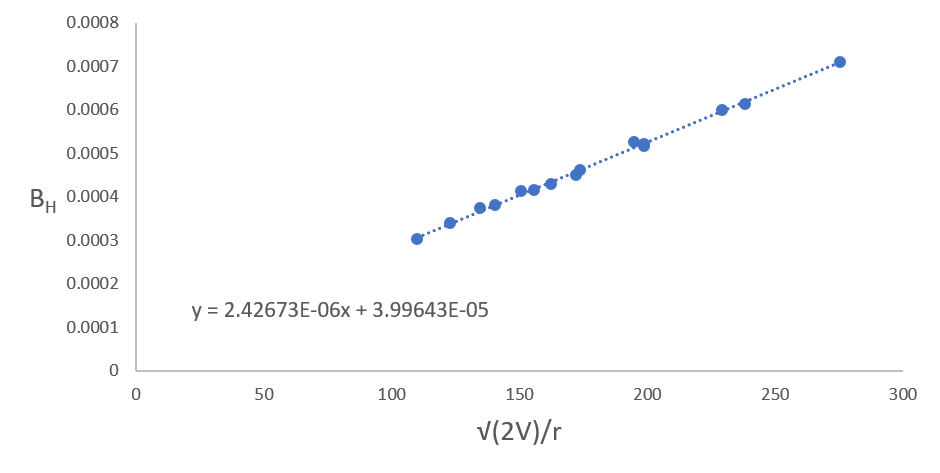
\includegraphics[width=\textwidth]{chart1.png}
  \caption{Measuring the voltage difference in a region between two parallel conductors.}
\end{figure}
\newpage
\noindent Using Excel's LINEST function, we obtain the following data from the graph in Figure 3.
\begin{table}[H]
\centering
\begin{tabular}{cc}
  Slope $\sqrt{m/e}$ : &  $\num{2.4267255938411E-06}\pm \num{3.50649774570897E-08}$ \\
  Y-Intercept $B_E$   :&  $\num{3.99642631798173E-05}\pm \num{6.40167504007098E-06}$ \\
\end{tabular}
\caption{LINEST data from the graph in Figure 3}
\end{table}

\noindent To obtain the calculated value for $e/m$, we can see from our LINEST data (Table 2) that the slope, $\sqrt{m/e}$ is
$\num{2.4267255938411E-06}$.\\
Thus, the calculated value of $e/m$ can be found:
$$ \frac{e}{m} = \left(\sqrt{\frac{m}{e}}\right)^{-2} = 1.69808200223924714236 \times 10^{11} $$
And the error $\delta \frac{e}{m}$ can be calculated using partial derivatives:
$$slope= \left(\frac{e}{m}\right)^{-1/2}$$
$$\delta slope = \left| -\frac{1}{2} \left(\frac{e}{m}\right)^{-3/2} \delta \left(\frac{e}{m}\right)\right|$$
$$ 2 \times \delta slope = \left(\frac{e}{m}\right)^{-3/2} \delta \left(\frac{e}{m}\right) $$
$$ \therefore \delta \left(\frac{e}{m}\right) = 2 \times \delta slope \left(\frac{e}{m}\right)^{3/2}$$
From our LINEST data (Table 2), we know that $\delta slope = \num{3.50649774570897E-08} $
$$ \therefore \delta \left(\frac{e}{m}\right) = 2 \times \num{3.50649774570897E-08} \times (\num{1.69808200223924714236e11})^{3/2}$$
$$= \num{4.90728801640585e9} \approx \num{4.91e9}$$
Thus, the calculated value for $\frac{e}{m}$ is:
$$\frac{e}{m}=\num{1.70e11} \pm \SI{4.91e9}{\coulomb\per\kilogram}$$
The percent error is:
$$ \frac{|\num{1.69808200223924714236e11}-\num{1.76e11}|}{\num{1.76e11}}\times100 = 3.52\%$$
Obtaining the calculated value and error for $B_E$ is a much simpler matter. We simply
look at the data generated by LINEST (Table 2).
$$B_E = \num{4.00E-05}\pm \SI{6.40E-06}{\tesla}$$
The percent error is:
$$ \frac{|\num{3.99642631798173E-05}-\num{4.8e-5}|}{\num{4.8e-5}}\times100 = 16.74\%$$

\vspace{1cm}
\noindent The calculated values of $e/m$ and $B_E$ from the graph are summarized in Table 3.
\begin{table}[H]
\centering
\begin{tabular}{c|c|c|c|}
                & Expected                      & Calculated:                                     & \% Error \\ \hline
$e/m$: & $\SI{1.76e11}{\coulomb\per\kilogram}$      & $\num{1.70e11} \pm \SI{4.91e9}{\coulomb\per\kilogram}$  &    $3.52$  \\ \hline
$B_E$: & $4.8 \pm \,\SI{0.3e-5}{\tesla}$           & $\num{4.00e-5} \pm \,\SI{6.40e-6}{\tesla}$                    &   $16.74$  \\ \hline
\end{tabular}
\caption{Measured values of $e/m$ and $B_E$ compared to the calculated values obtained from the graph.}
\end{table}

% \subsection{Part 2}
% % Part II\\
% % Provide graph from the template\\
% % By hand draw field lines, show charge
% % distribution, etc.\\
% % Provide the explanation, calculations,
% % answer questions in Discussion.\\
%
% Raw data recorded while measuring potential differences at various points on
% the parallel plate capacitor is given by Table 4. Each cell corresponds to one
% of the points on the grid as seen in Figure 3.
%
% % Please add the following required packages to your document preamble:
% % \usepackage{graphicx}
%
% \newpage
% From the above data, the following graph was generated in Figure X, which gives a visual representation of the electric
% equipotential lines on the capacitor.
%
% % \begin{figure}[H]
% %   \centering
% %   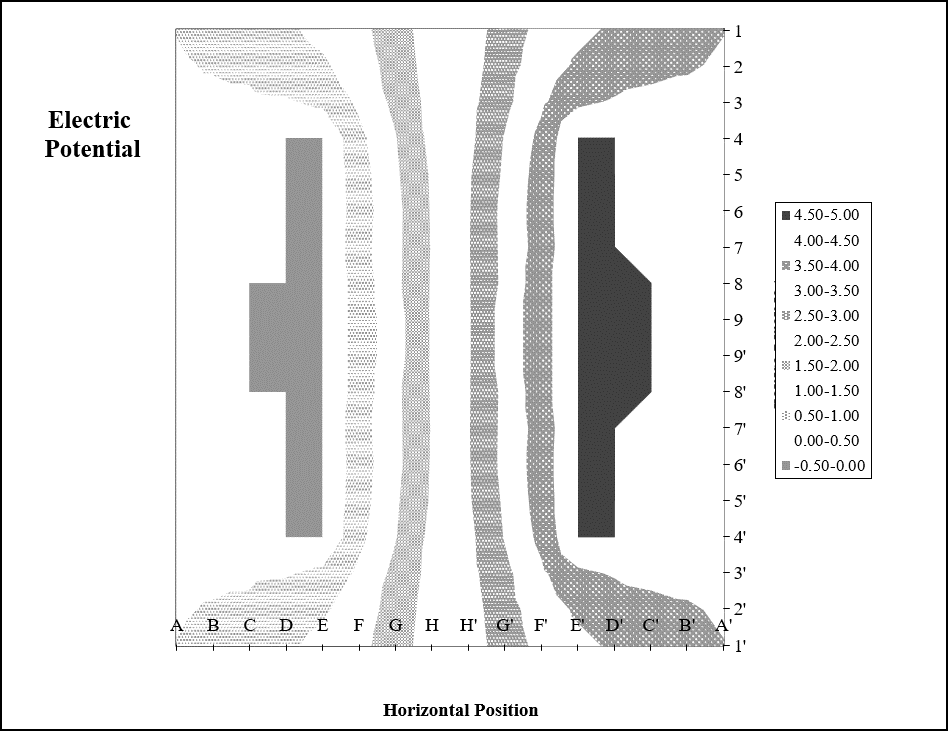
\includegraphics[width=.9\textwidth]{chart2.png}
% %   \caption{A visual representation of the electric equipotential lines between the plates of the capacitor. This figure was generated using the data in Table 4.}
% % \end{figure}
% % \vspace{2cm}
% % The next figure, (Figure 6) was also generated from the data in Table 4, which is a 3
% % dimensional plot of the potential difference at different points on the parallel plate capacitor
% % as a function of the horizontal and vertical positions of the probe.
% % \begin{figure}[H]
% %   \centering
% %   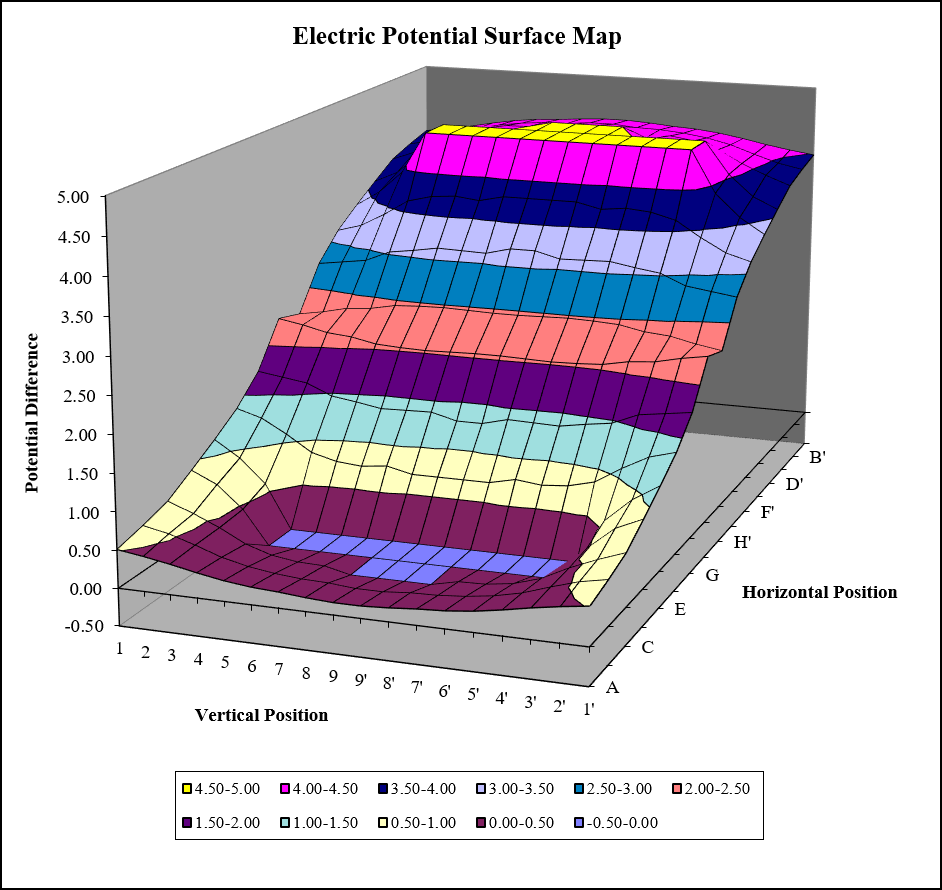
\includegraphics[width=\textwidth]{chart3.png}
% %   \caption{An electric potential surface map generated from the data in Table 4 above}
% % \end{figure}



\section{Discussion}

\subsection{Part 1}


From Table 3, we can see that our calculated values for $e/m$
($\num{1.70e11} \pm \SI{4.91e9}{\coulomb\per\kilogram}$)
and $B_E$
($\num{4.00e-5} \pm \,\SI{6.40e-6}{\tesla}$) were in the same order of magnitude as the
expected values. ( $\SI{1.76e11}{\coulomb\per\kilogram}$ for $e/m$
and $4.8 \pm \,\SI{0.3e-5}{\tesla}$ for $B_E$.)
Additionally, the percent error for the charge to mass ration seemed relatively good, being 3.52\%.
However, our calculated value of $B_E$ was a fair bit off, with a 16.74\% error.
Unfortunately, it is clear that our calculated values do are not within error of the
expected values.

At first glance, the graph (Figure 3) produced from our raw data (Table 1) seems reasonable, especially
because all the data points recorded seem to fit nicely on the trendline with
no anomalous data points compared to the other values. This means that whatever error
introduced in our measurement of voltages was a constant factor, since we took care
to measure the currents exactly when the electron loop was on the far side of each peg, as specified in the
lab manual.There are many potential sources of error, including human error, and potential miscalibration of equipment since we are dealing
with electrons which are tiny in nature. We did our best to keep these factors constant.

Using the left-hand-rule for moving charge (since we are
dealing with electrons which have a negative charge), we determine that the net magnetic field \textbf{B}
points upward, perpendicular to the radius of the coil, or upwards relative to Figure 2.

Equation 1, which which was manupilated to produce our graph can be derived using the following equations:

\noindent When a stream of electrons are accelerated through a potential difference $V$, the maximum
kinetic energy is given by:
$$\frac{1}{2}mv^2 = eV$$
Next, the Lorentz force \textbf{F} is given by:
$\textbf{F}=q\textbf{v}\times \textbf{B}$
and since our magnetic field is set up so that \textbf{B} is perpendicular to the motion of the electrons (see Figure 1),
the magnitude of the force $F$ is given by $$F=qvB$$
Next, the radius of the circle, which is the path of the electrons in this experiment is such that
the centripetal acceleration is furnished by the Lorentz force. Therefore, we obtain $$\frac{mv^2}{r}$$.

\noindent To obtain Equation 1, we first rearrange the first of the three equations above and substitute it into the third.
$$\frac{1}{2}mv^2 = eV \Rightarrow v=\frac{\sqrt{2eV}}{m}$$
$$\Rightarrow \frac{m(\frac{2eV}{m})}{r}=e\sqrt{\frac{2eV}{m}}B$$
$$\Rightarrow \frac{4V^2}{r^2}=\frac{2eV}{m}B^2$$
$$\Rightarrow \frac{e}{m} = \frac{2V}{r^2B^2}$$
Finally, we notice that since our apparatus is aimed antiparallel to earth's magnetic field, such that
the magnitude of the total magnetic field $B=B_H-B_E$, and substitute this result in the above equation.
Finally, we obtain equation 1.
$$\frac{e}{m} = \frac{2V}{(B_H-B_E)^2r^2}$$


% \subsection{Part 2}
% From figure 5, we can see how the equipotential lines along the capacitor show that the
% electric field close to the center of the parallel plate capacitor is almost uniform, and
% how we get fringing effects towards the edges of the capacitor, which make the electric field non uniform
% in that area. This aligns well with what we have learned so far in the lecture part of this course.
% \\ \\
% The magnitude of the electric field is strongest where the equipotential lines are the closest.\\
% Using equation 1 with cells E4 and F4 in Table 4,
% $$ E=-\frac{\Delta V}{\Delta s}= -\frac{0.87 V -0.00 V}{0.95\times 10^{-2} m} = -91.58 \:V/m $$
% \\ \\
\textbf{Questions: }\\ \\
\textit{Why is it important to align the Helmholtz coil, so that its field is
        anti-parallel to the earth's magnetic field?}\\
\textbf{A:}
Earth's magnetic field is strong enough to deflect our little electron beam\\ \\
\textit{Explain what would happen if the beam in this experiment contained several ions of different masses.}\\
\textbf{A:}
biggermass means larger radius of curvature

\section{Conclusions}
In Experiment 1, we first measure potential differences at various radii on a circular capacitor,
and use Gauss's Law to calculate the inner and outer radii of the capacitor. We then check these predictions
by physically measuring the inner and outer radii of the circular capacitor. Although our data seemed
fine, our calculations did not agree within error of the measured values. Our inner radius was calculated to be
$1.73 \pm 0.03 cm$, while our measured value was $1.9 \pm 0.1 cm$, and the outer radius of the circular capacitor
was calculated as $9.3 \pm 0.1 cm$, while the measured value was $9.5 \pm 0.1 cm$. Since our resulting graph (Figure 4)
was linear as expected. with no anomalous data points, the source of error was a constant factor, and therefore can
likely be attributed to a faulty voltmeter. It should also be noted that when measuring the potential differences, pressing
the probe on the capacitor with varying pressures and angles could change the measured potential difference.
We did our best to keep these factors constant by taking multiple measurements.

Next, we measured potential differences at various points on a parallel plate capacitor, and used the data to generate
a graph which allows us to visualize the equipotential lines. The same data was also used to generate a 3 dimensional
surface plot of the potential differences as a function of the horizontal and vertical position of the probe on the parallel plate
capacitor. This allows us to visualize the electric potential on the capacitor.
  % In lab 8, we set up a pendulum with a 2.3kg bob hanging off of a string, and put an arced track such that the bob would be close enough to the track at any point while it swings to make a spark, with a spark timer. We then used an electromagnet to release the bob from rest, and used the spark timer to keep track of the bob’s displacements, and since the spark timer sparks at regular intervals, we had enough data to generate plots in Excel of potential energy, kinetic energy, and total energy as functions of time. The law of conservation of energy says that energy cannot be created or destroyed, but it can be converted. Theoretically, all of the Pe at the beginning should convert completely into KE, and then towards the end, all of the KE that the bob has should convert back into PE. Indeed, we do observe this behaviour in the lab, albeit not perfectly, since energy is also lost due to some of it being converted to other forms such as friction. This caused TE to decrease over time. Additionally, there were some anomalous data points that can be attributed to the spark timer missing sparks. Overall, however, the data seemed reasonable, albeit the amount of energy lost per second using the graph’s data versus taking an average after 25 periods did seem to disagree with 3 orders of magnitude.  One can observe the physics principles explored in the lab in real-life such as on a rollercoaster, where the gravitational potential energy is also converted into kinetic energy and vice versa such as when the car is going through a loop.
\bibliography{references}
\end{document}
